\chapter{UML Models} \label{chap5}

\section{Use Case Diagram}
The Figure \ref{fig:usecase} gives an overview on the main actors involved in the system and the functionalities that they are able to execute.

\begin{figure}[htbp]
\centering
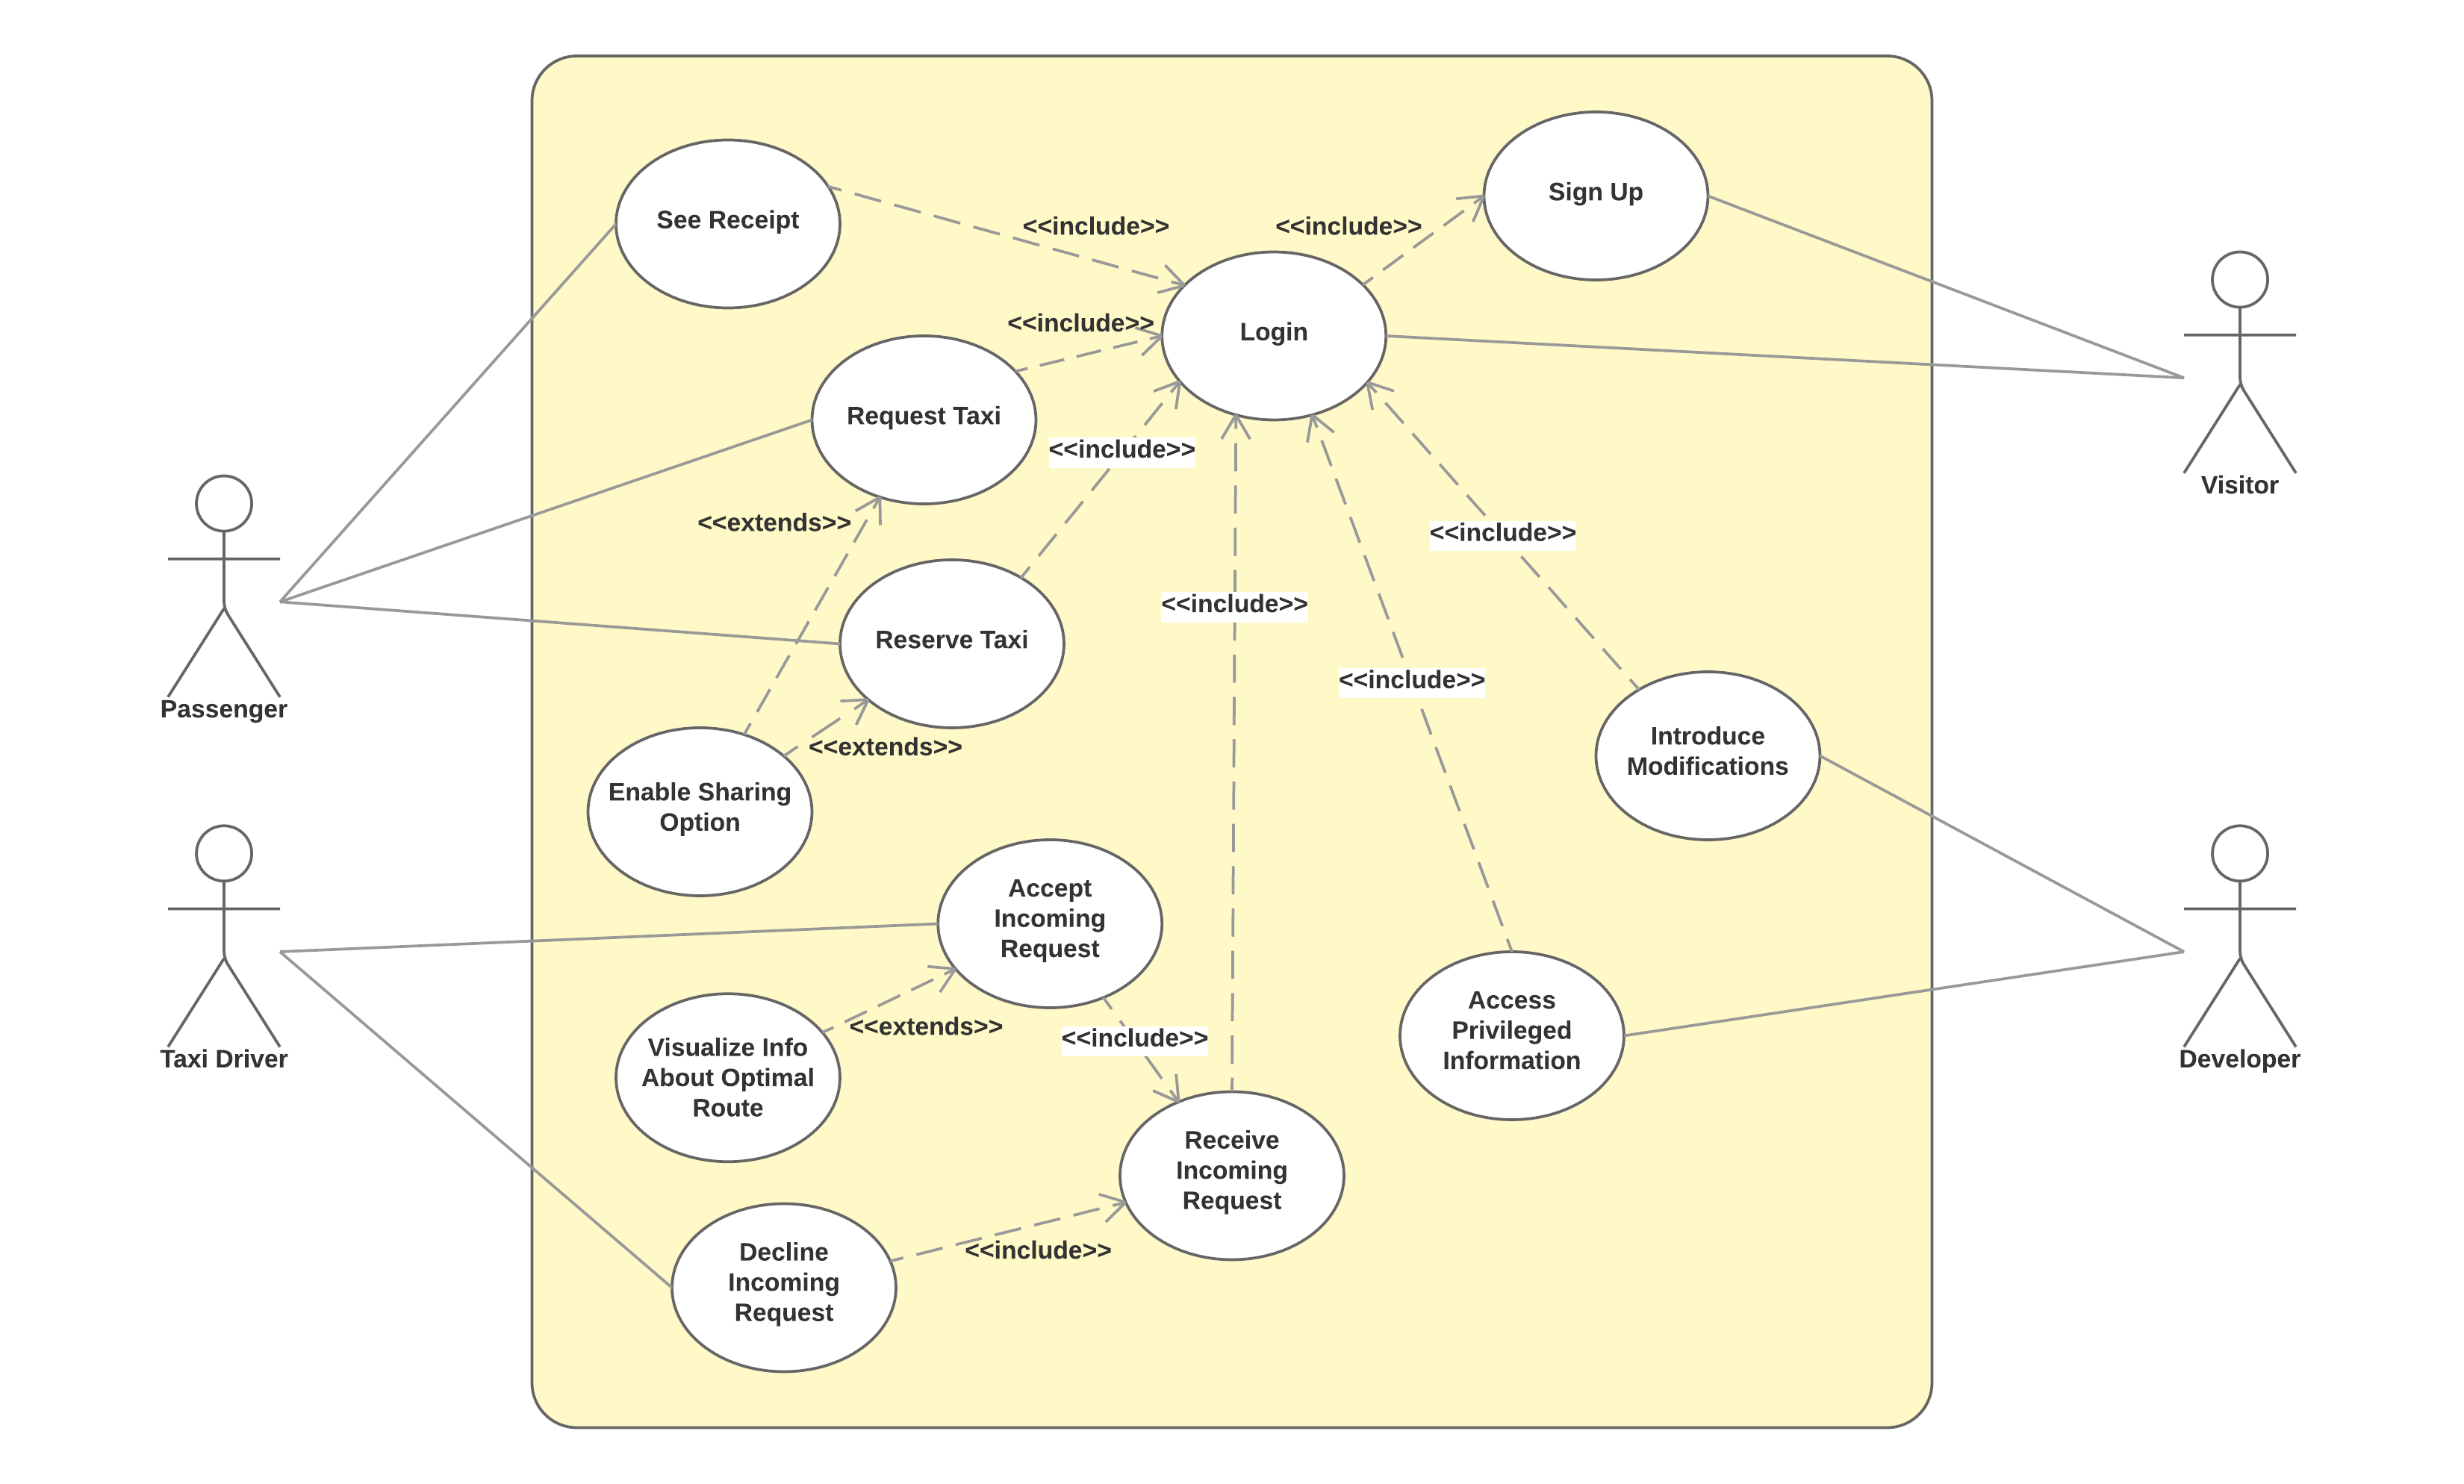
\includegraphics[width=\textwidth]{cpt/img/UseCase}
\caption{Use Case Diagram}
\label{fig:usecase}
\end{figure}

\section{Use Case Description}

\subsubsection{Sign Up}

\subsubsection{Login}

\subsubsection{Request Taxi}

\subsubsection{Reserve Taxi}

\subsubsection{Enable Sharing Option}

\subsubsection{See Receipt}

\subsubsection{Accept Incoming Requests}

\subsubsection{Decline Incoming Requests}

\subsubsection{Receive Incoming Requests}

\subsubsection{Visualize Information About Optimal Route}

\subsubsection{Introduce Modifications}

\subsubsection{Access Privileged Information}

\section{Class Diagram}
Here is presented the UML class diagram in Figure \ref{fig:classdiag}. This diagram will be updated during the developing process especially by adding all methods:

\begin{figure}[htbp]
\centering
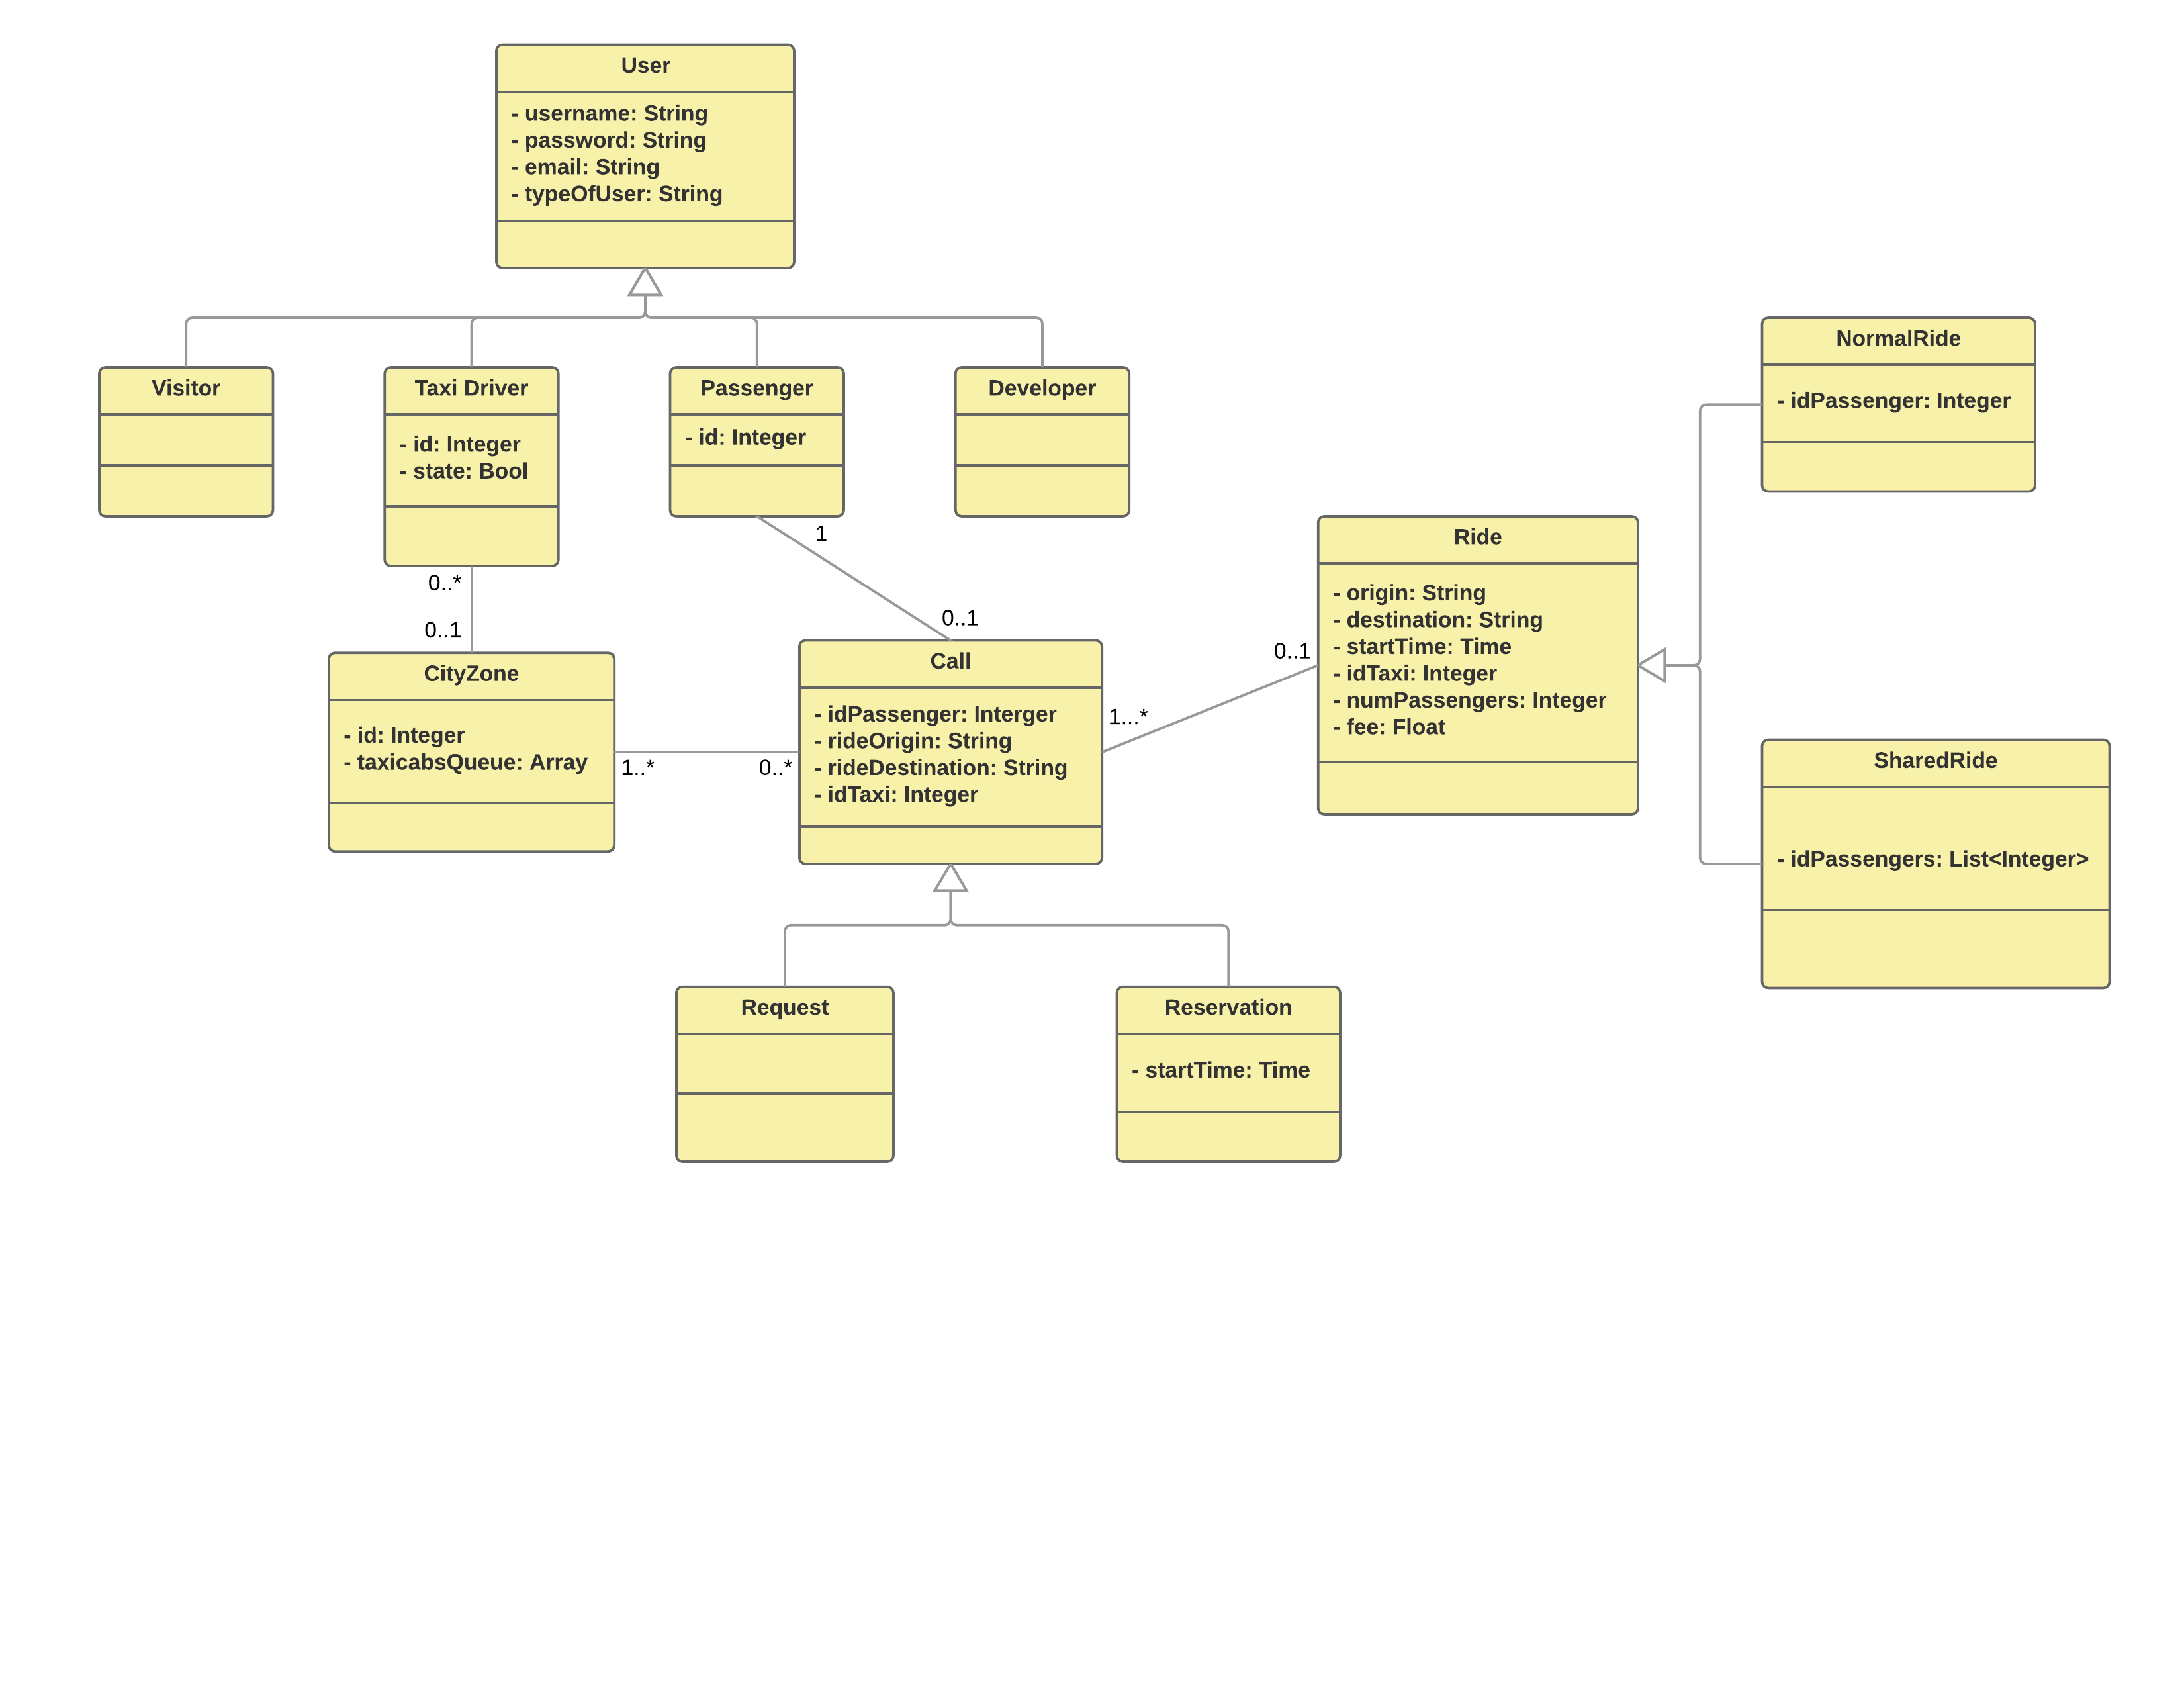
\includegraphics[width=\textwidth]{cpt/img/ClassDiagram}
\caption{Class Diagram}
\label{fig:classdiag}
\end{figure}

\section{Sequence Diagram}

\subsubsection{Log In}

\subsubsection{Request a Taxi Ride}

\subsubsection{Reserve a Taxi Ride}

\subsubsection{Introduce Modifications in the System}

\section{State Chart Diagram}
In this section the behavior of some entities presented in Figure \ref{fig:classdiag} is exposed using UML state chart diagrams. The following state chart diagrams will give a simplified vision of entire application:

\subsubsection{State Chart Diagram for Passengers}

\begin{figure}[htbp]
\centering
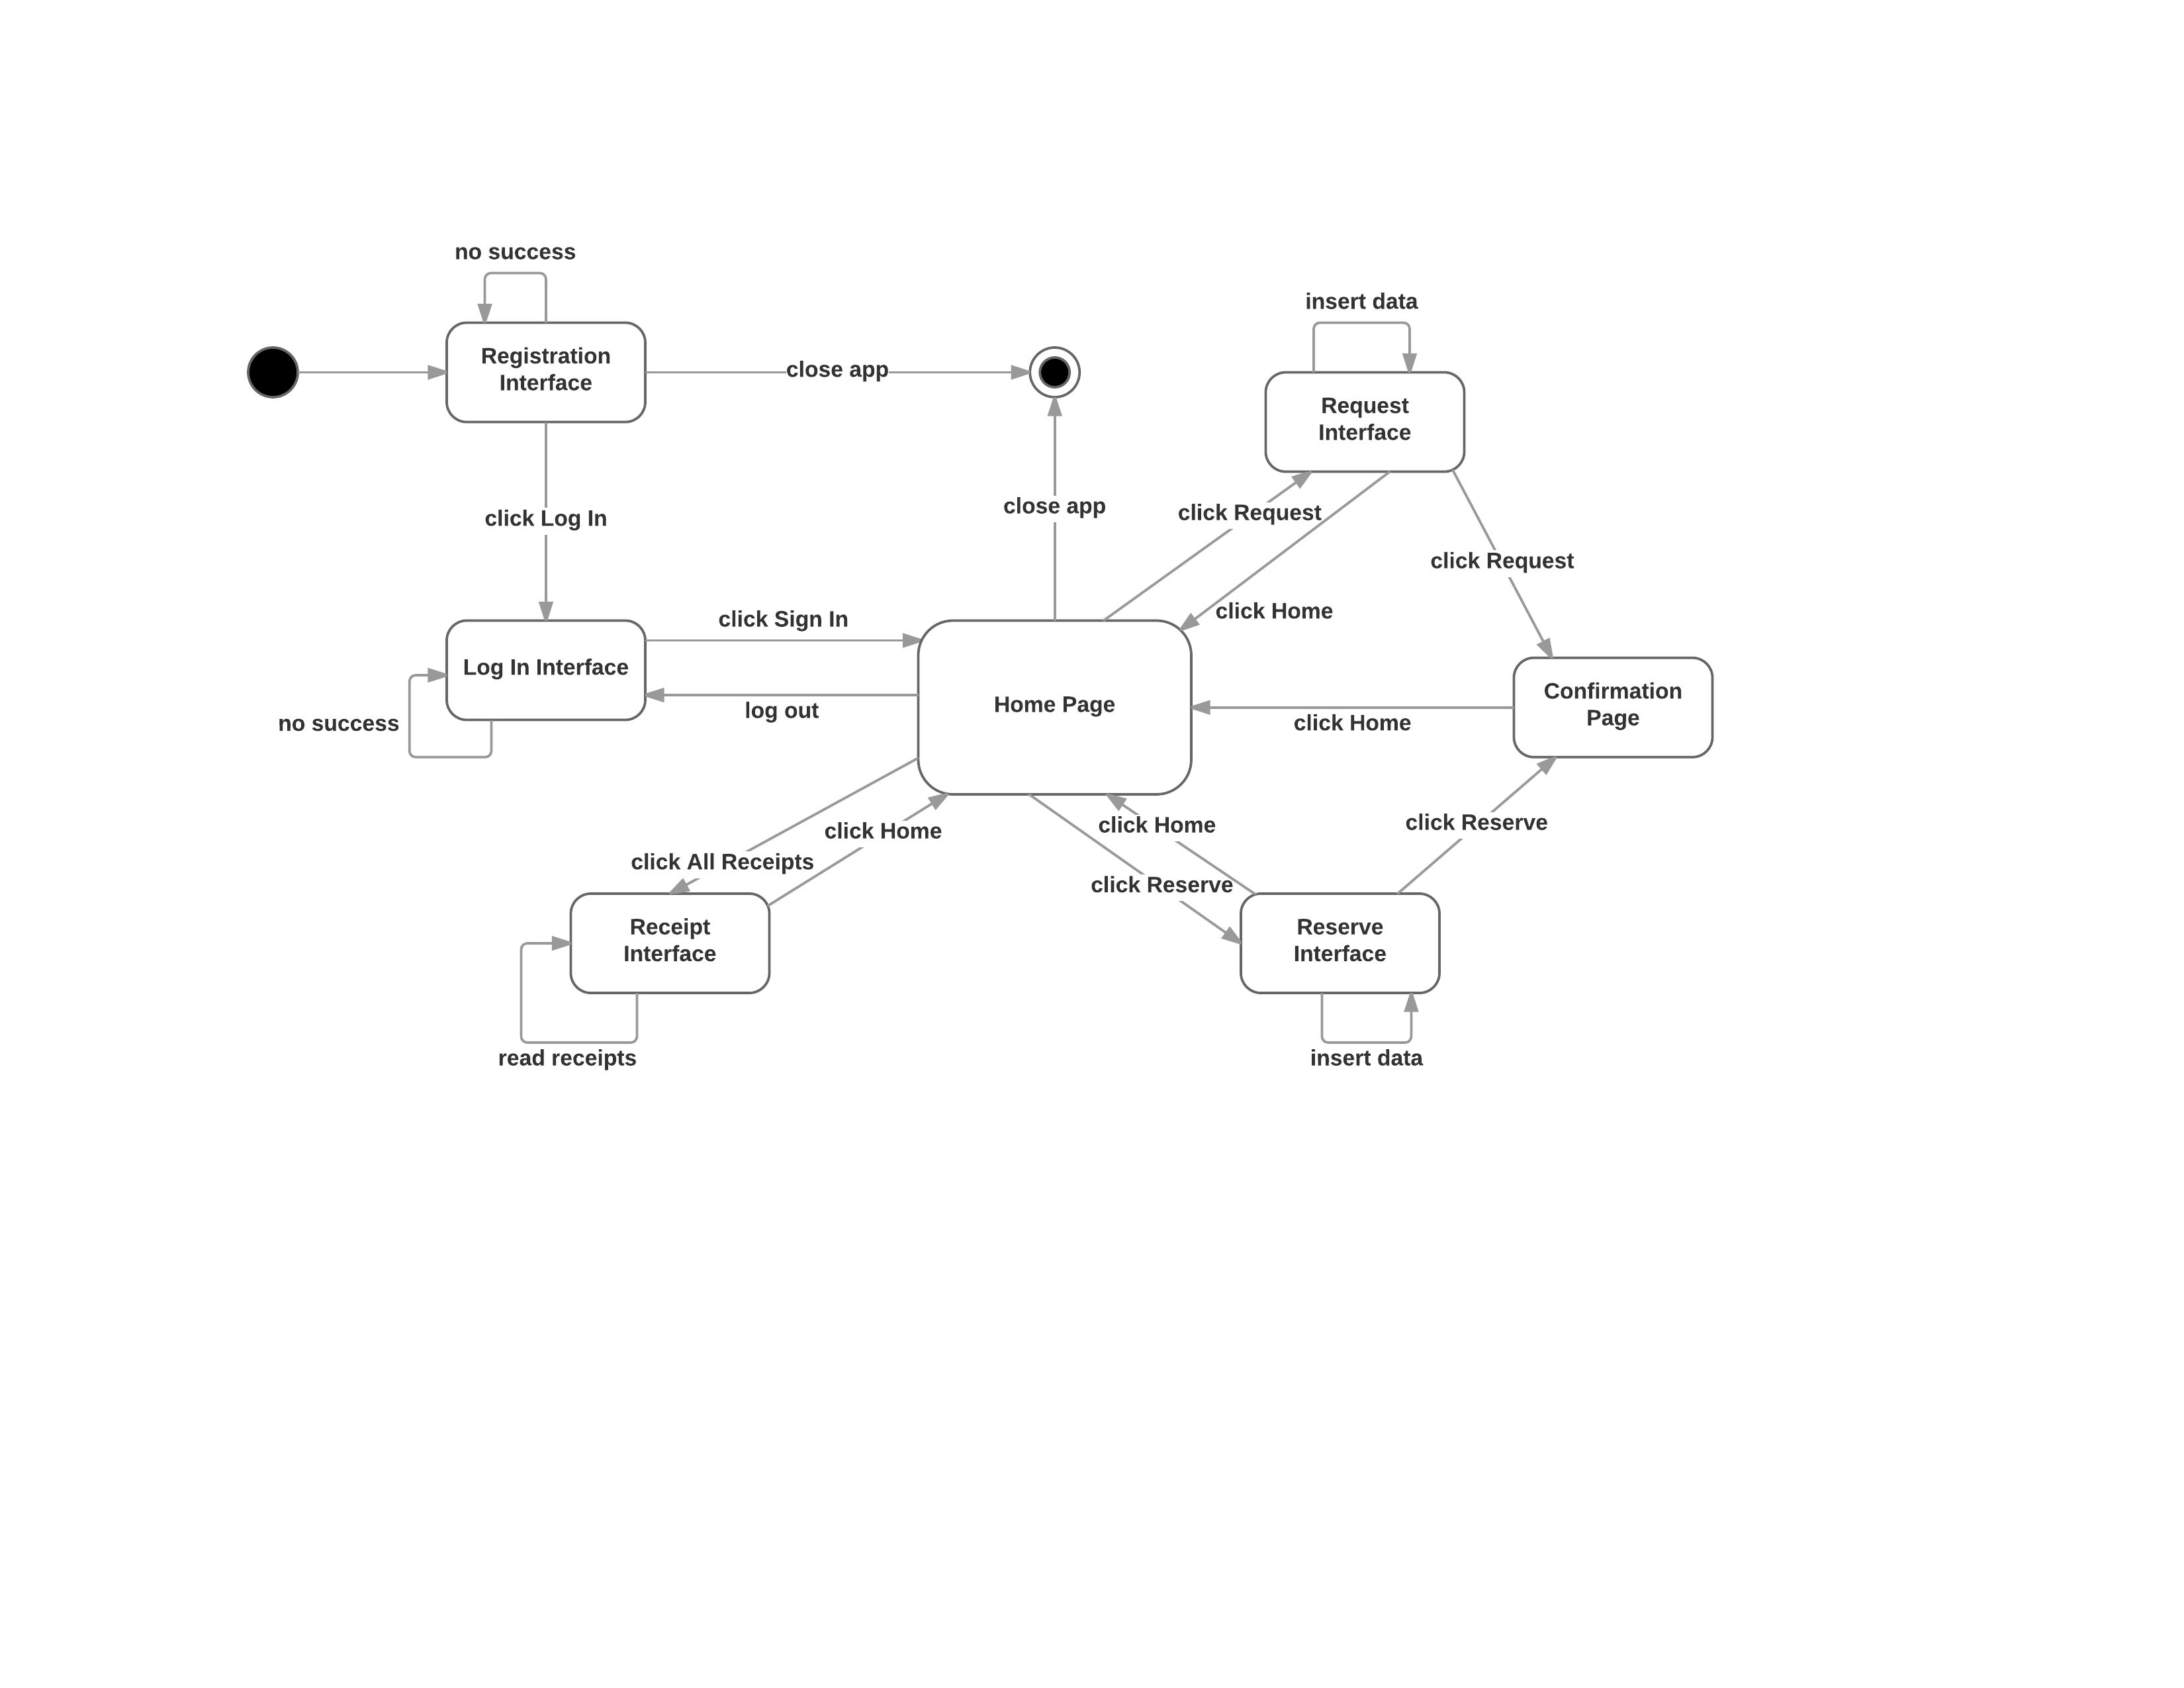
\includegraphics[width=\textwidth]{cpt/img/StateChartPass}
\caption{State Chart Diagram for Passengers}
\end{figure}

\subsubsection{State Chart Diagram for Taxi Drivers}

\begin{figure}[htbp]
\centering
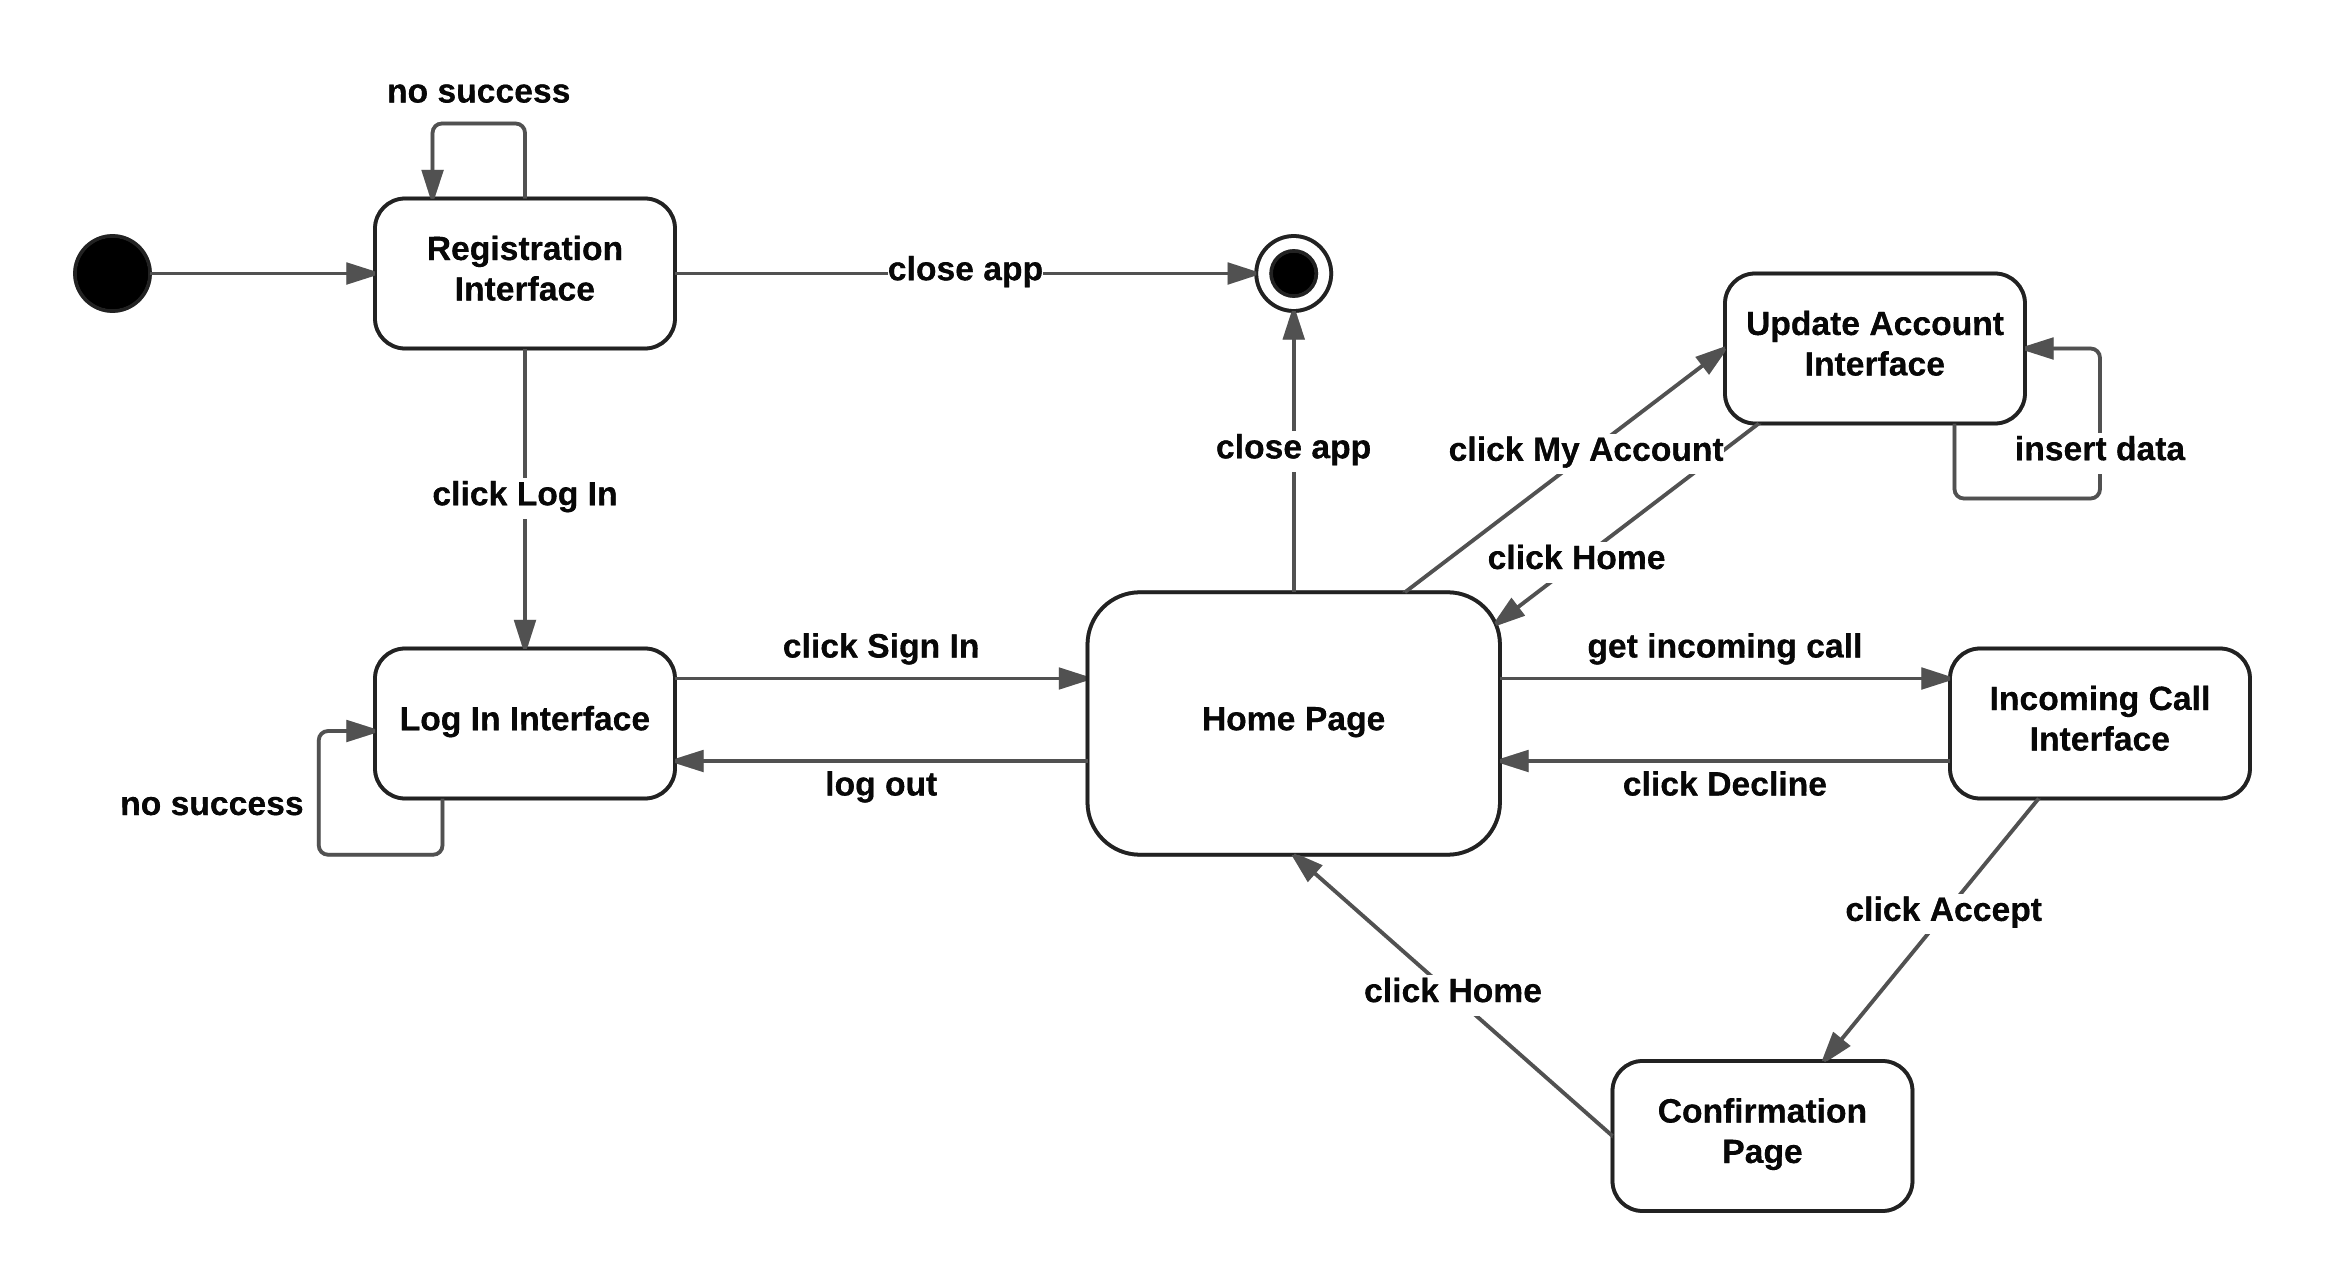
\includegraphics[width=\textwidth]{cpt/img/StateChartDriver}
\caption{State Chart Diagram for Taxi Drivers}
\end{figure}